\section{Mediciones}

Se realizaron medicions en base a crear arreglos de diferentes largos, yendo de 100 en 100 elementos, donde los elementos en cada caso fueron generados por los valores pseudoaleatorios del lenguaje (el módulo \texttt{random}). 

\begin{figure}[H]
    \centering
    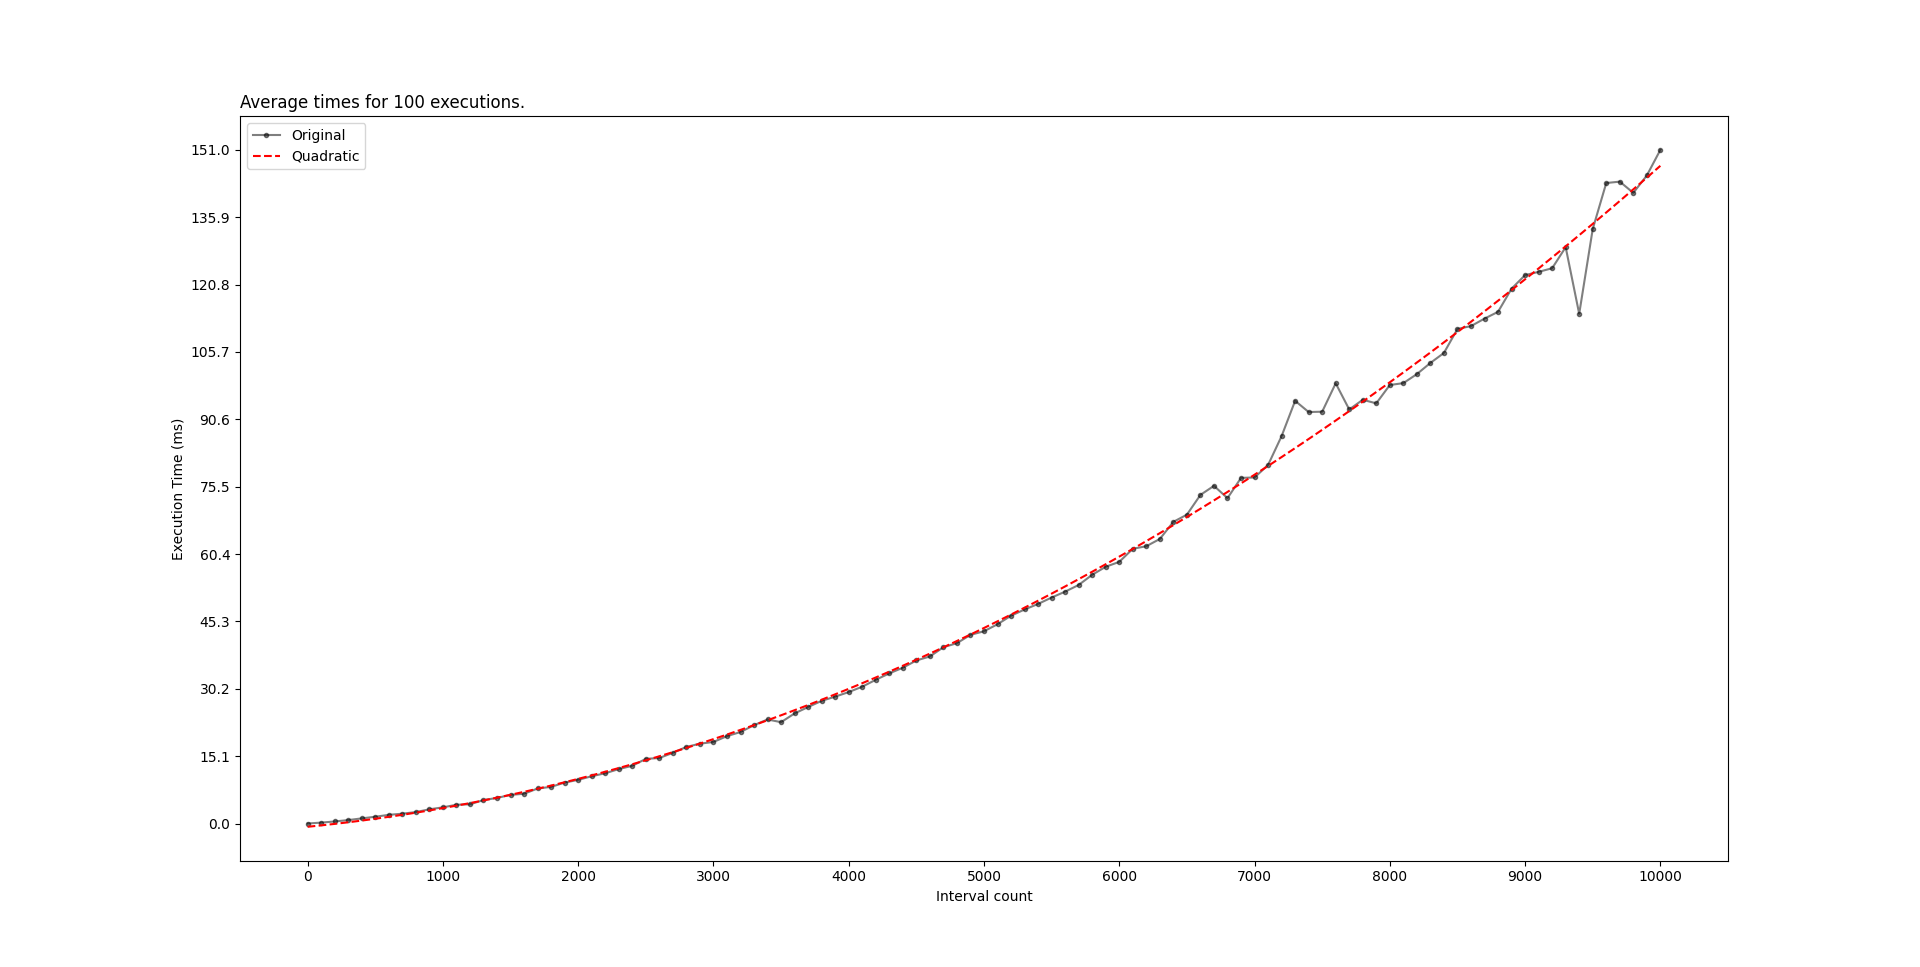
\includegraphics[width=1\textwidth]{../images/graphic_100Intervals.png}
    Este gráfico muestra el tiempo de ejecución promedio de 100 ejecuciones del programa (en milisegundos) dada una cantidad de intervalos con un acomodo cuadrático
\end{figure}

\begin{figure}[H]
	\centering
	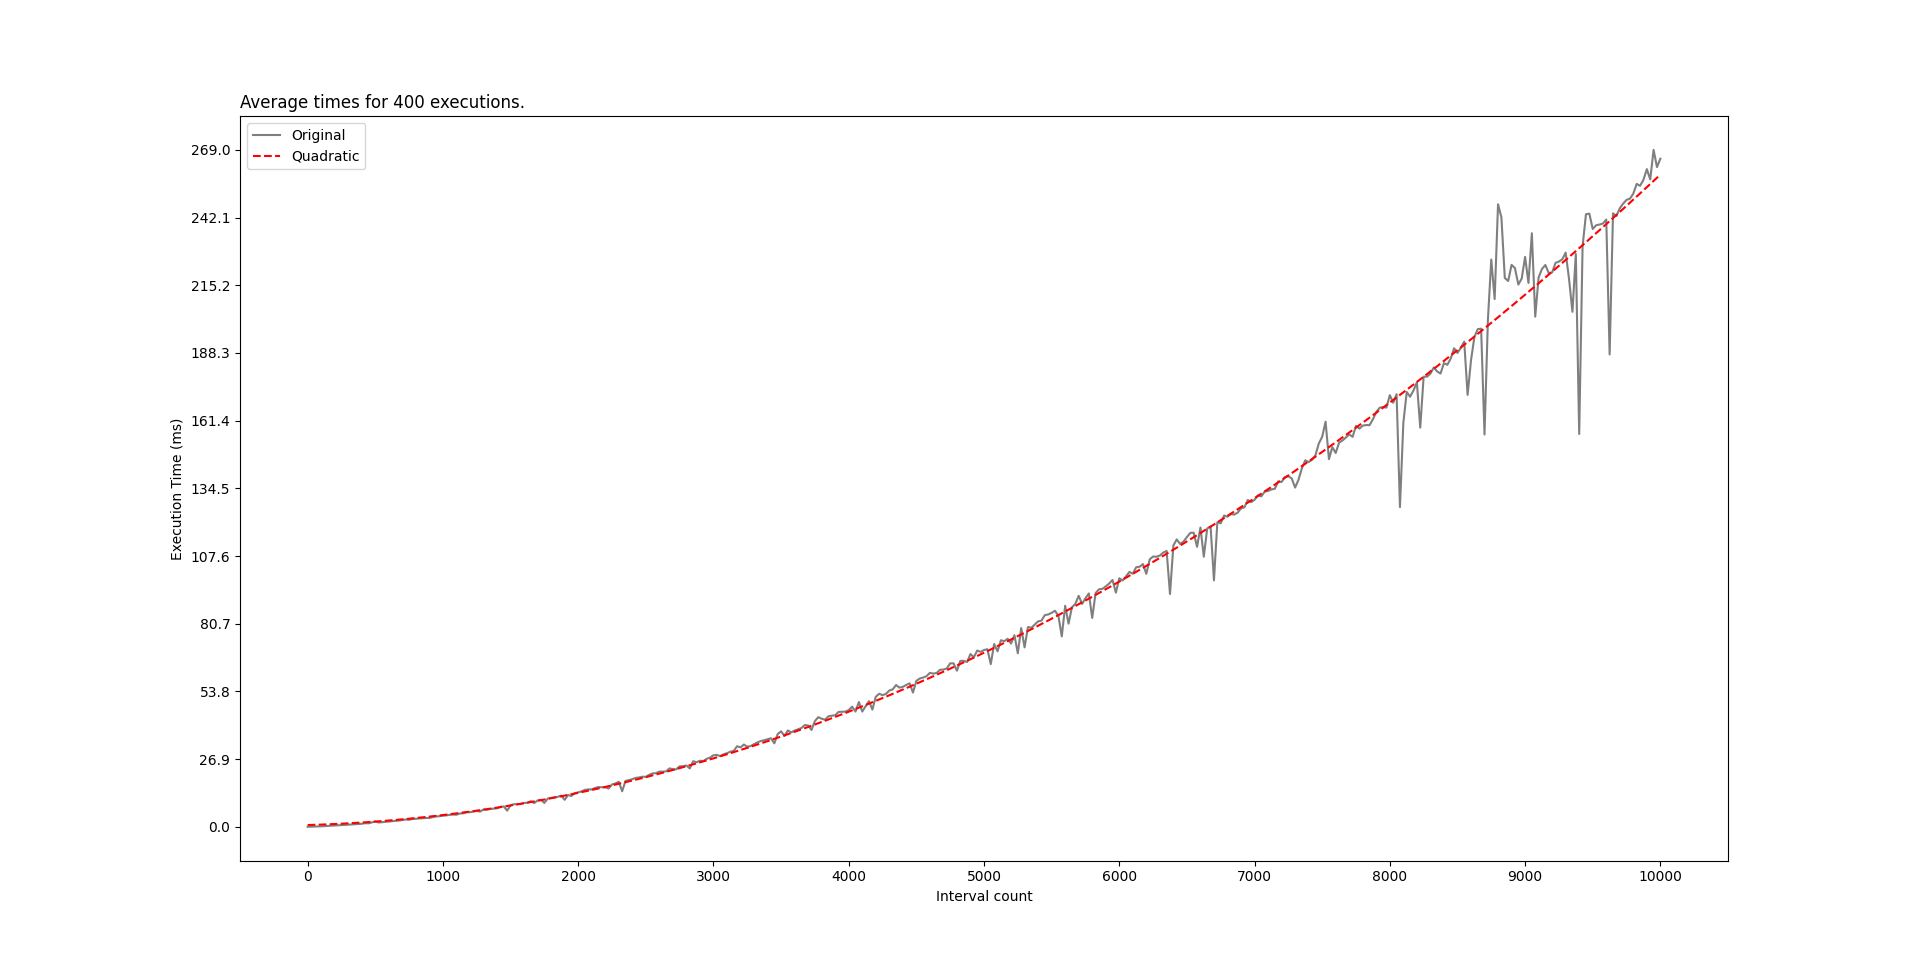
\includegraphics[width=1\textwidth]{../images/graphic_400Intervals.png}
	Este gráfico en cambio muestra el tiempo de ejecución pero del promedio de 400 ejecuciones del programa (en milisegundos)
\end{figure}

Como se puede apreciar, el gráfico muestra una tendencia cuadrática como lo explicado en el análisis de complejidad
